\documentclass{amsart}
\usepackage{amsmath}
\usepackage{upgreek}
\usepackage{amssymb}
\usepackage{graphicx}

\usepackage{enumerate}
\usepackage[utf8]{inputenc}

\usepackage{tikz}
\usepackage{hyperref}

\setlength{\textwidth}{6.37in}
\setlength{\marginparwidth}{0pt}
\setlength{\evensidemargin}{0in}
\setlength{\oddsidemargin}{0in}

\newtheorem{theorem}{Theorem}[section]
\newtheorem{conj}[theorem]{Conjecture}

\usepackage{titling}
\setlength{\droptitle}{-8em}

\title{CS 452 Train Control One \vspace{-0.65cm}}
\date{Louis A. Burke (laburke) and Taras Kolomatski (tkolomat)}

\begin{document}

\maketitle

\begin{center}
\vspace{-0.58cm}
June 29\textsuperscript{th}, 2017
\end{center}

\section*{Overview}

\textsc{When} I was seven years old, I set out one day determined to discover whether on not I possessed telekinetic abilities. The conjecture was, as I outlined to myself at the time, that, noticing my decreasing level of clumsiness, one makes gestures more from memory and less from improvisation as one ages, hence the absence of this skill in adults could be explained by their being remiss to preform these experiments while young. I sat in my room and stared at objects, harbouring an intense psychological desire and focus that any \textit{fair} universe would reward by yielding its control to my mind. \textit{Nothing moved}.

The universe is apathetic to desire or expectation. One cannot wish a object or event into existence. It would seem that the conclusions I ought to have drawn from this investigation, paralleling the general disillusionment of childhood na\"ievity upon entering the adult world, would have been that the human mind is feeble and that functional living comes only from imitating the social motions of society, accidentally designed by eons of trial and error.

The lesson I learned, however, was starkly different. Suppose a benevolent universe, concerned with human life, were in place. Then the stability of an architecturally daring skyscraper, the precision of an engine, the intricacy of microchips, and the accuracy of statistical models for high energy physics, all could be handouts from the actual powers that be. Abandoning this hypothesis leads to the conclusion that mind is in fact able to modify the universe in unprecedented ways, and has at an increasing pace through history.

Through it's uncaring nature, bending to the will of no man, the universe is able to produce regularity. The task of mankind is to discover regularity, and through ingenuity, permit a three pound organ, consisting largely of fat, to shape the world through thought alone.

In the first train control milestone, we produced an accurate model of stopping distance that was defined by only two parameters (and the provided distance data).

\section*{The Experiment}


Entering this project, we were adamant that no rote measurements would be made. Particularly, if we admit that the problem of determining velocity is solved (at least in steady state), a solution to the problem of stopping a train at a given location requires solving the problem of stopping distance, thus we required a way to measure stopping distances without the use of a tape measure. The only situation in which we know the location of a train to high precision is while it is over a sensor. Thus the natural way to automate collection of stopping distances is to stop the train exactly on a sensor. We recorded the number of ticks that separated the last sensor activation and the issuing of the stop command, this allowed us to approximate the position of the train at the time of the stop command from velocity data (these were on the order of 10cm past a sensor, which is small relative to the observed stopping distances, thus allowing for error in the velocity prediction). From the distance data, this would allow us to record stopping distance within a few centimetres. This motivated us to reformulate the goal of this assignments as to be able to stop at a switch, as this problem is most well defined in the code.

Out testing program would take two points, route and flip switches as to form a loop, make a reasonable estimate of what delay after sensor A would issuing a stop command at result on the train resting a point B, determine whether we undershot or overshot, and adjust the delay, such that by trail end error we would get a data point. Impatience with waiting for results drove us to narrow our heuristic for reasonable estimates.

Initially, we wanted to eliminate acceleration from standstill and chose to run the loop for one full cycle before issuing a stop command. We found that the distances from point B to A that we were working with were sufficient to place the train in a steady state at the time it came to A after stopping (as seen by inter-sensor delays). Thus we eliminated all intermittent full loops, less the first, which served to gather velocity data over its full length to determine the initial estimate. We initially adjusted delays by 10 ticks on failure and would experience two errors prior to a success at general positions.

\textbf{Full disclosure}: \textit{Of the 60 data points used to generate the following graphs, five starkly outlying points were pruned from the data}.

The first set of data that we compiled was for stopping distances to the sensor B2 on track A with train 70 at different speed settings. The independent variable was the incoming velocity measured over the two (justified by the desire to remove noise from data, as motivated by an careless invocation of the central limit theorem) full segments before the one in which the stop command was issued. The results were as follows:
\begin{center}
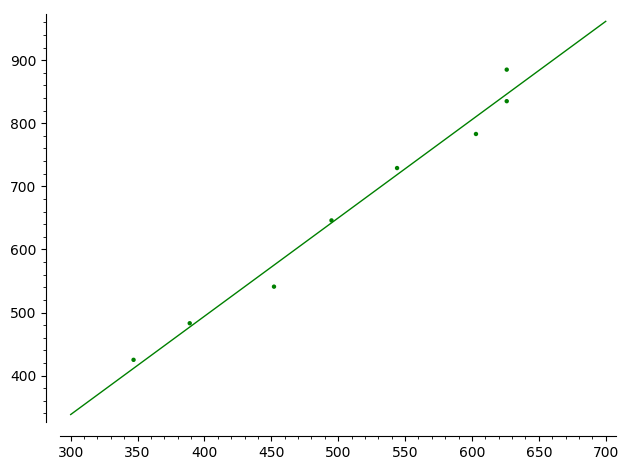
\includegraphics[scale=0.5]{x17s}
\end{center}
In our first observation run, we fond compelling evidence that stopping distance had a linear relation with incoming velocity. We repeated this experiment for a number of other locations on the track and compiled the data as follows:
\begin{center}
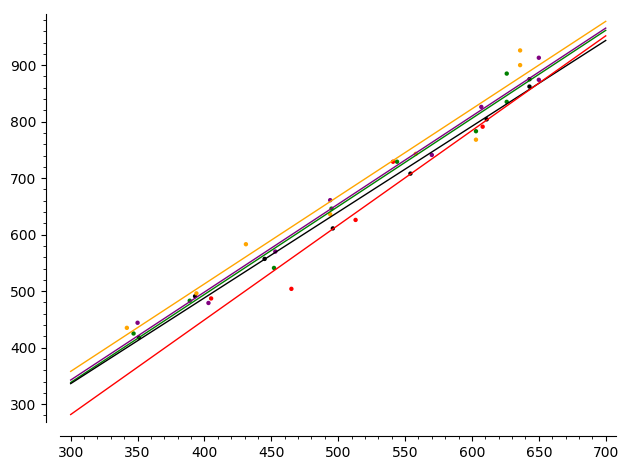
\includegraphics[scale=0.5]{all}
\end{center}
This suggests that the \texttt{a} parameter of $ax+b$ linear regressions at each point is reasonably uniform across the track.

Fitting parameters from the first regression improved our heuristics for a small number of points to correct within ~15 ticks, on average. The above plot was actually made nearer to the end. Our second experiment was to alter the stopping location and to keep the set speed (10) constant. We obtained the following plot:
\begin{center}
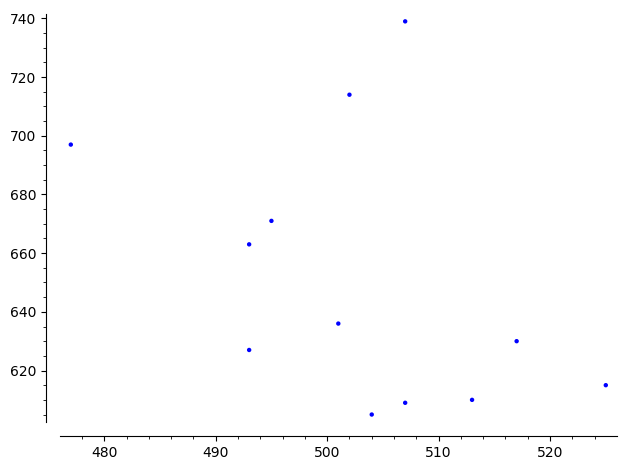
\includegraphics[scale=0.5]{x10s}
\end{center}
This either looks random, or strongly negatively correlated when two points are omitted. It was at this point that we gathered readings ranging over sensors and speeds, spanning an hour and a half of automated testing. We plotted the data to obtain the following:
\begin{center}
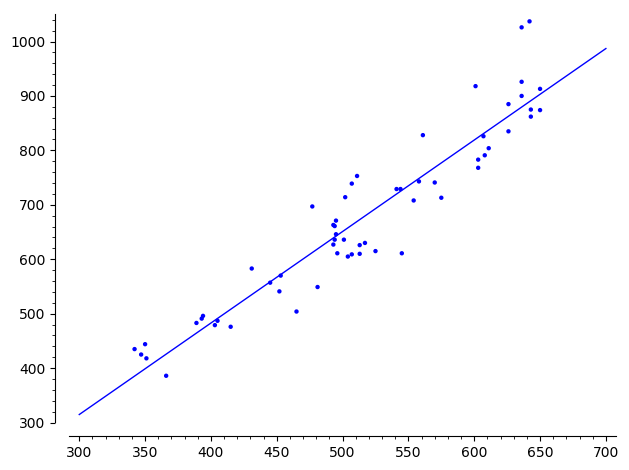
\includegraphics[scale=0.5]{regression}
\end{center}
At lower speeds, there is strong evidence of an inverse relationship between incoming speed and stopping distance within each speed class! Thus if we demoed at only one speed, as we did (because it was hard-codded; more on that later), the overall regression would not serve us at all. It would in fact be much worse than our heuristic estimates, which were at this point based off of the last four (joint incoming and outgoing) velocities observed in the calibration loop.

At this point, the investigation became difficult and proceeded down many barren paths. Generally, we were aware that track conditions of the section that we were stopping on should determine the deceleration curve. However, we thought that the incoming velocity was to be a central part of the model. We considered ratios of incoming to outgoing (over the two segments over which the stopping occurs) velocities in the calibration loop. There was no clear joint relationship between the incoming velocity, the ratio, and the stopping distance (we hoped for a $vr^\alpha+b$ model).

\clearpage

Finally, after trying out many sets of variables, we plotted stopping distance relative to that over the two outgoing segments in the calibration loop. We got the following graph:
\begin{center}
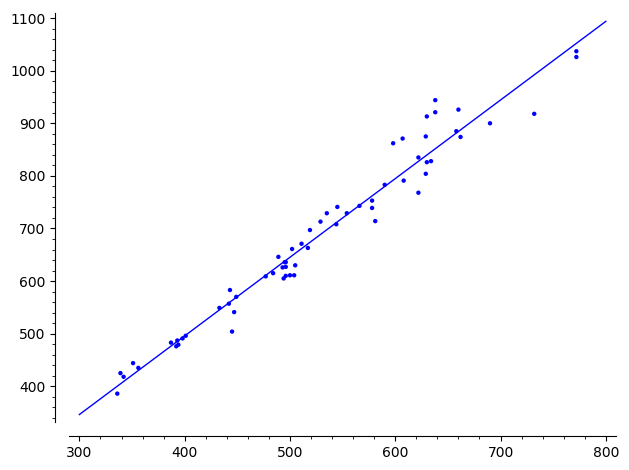
\includegraphics[scale=0.5]{solution}
\end{center}
This was a remarkable fit! We proceeded to test this model in our testing program and were able to consistently land exactly on the sensor in more then half of the cases, or at most with $<5$ ticks of correction otherwise. This held of sections of the track that we had never passed over in the tests on which the model was based. Hence one would expect this model to work as well on track B as track A.

\section*{Analysis}

We observed that speed over outgoing segments correlates very strongly with stopping distance. Let's begin by narrowing down on the definition of the independent variable. We began from steady state, by the construction of the interlacing tests, prior to point B, as such, the measurements made on the calibration loop, being the velocities measured on the route from A to B, were made in the steady state. If the train had acceleration or deceleration that was not attributed to solely track topography, the statistical evidence we have amassed would not apply.

\begin{conj}
In the steady state, the velocity is able to adjust to reflecting track topography sufficiently rapidly, as such, track quality is accurately reflected by velocity in the steady state.
\end{conj}

Notice that the relationship in the previous graph has no clear separation between speed classes, so it appears that steady state velocity is predictive, even uniformly across different steady states. The work being done by the train's motor is not required for completeness of the description, this is very surprising.

What is more surprising is that there is a negative correlation between steady state velocities on adjacent pieces of track! We have not yet investigated this relationship to a satisfactory extent. However, we can say that it is not a matter of where on a bar the sensor hits. Velocities on segments, with the same pattern of highs and lows, remain while running the train multiples times over the same loop, as tried on several loops. It would be very unlikely that distances would be exactly consistently distorted by the train hitting one sensor with the tip of its contact tip as opposed to the tail. This would explain the negative correlations between adjacent sensors in one run. However, the plot is made with respect to incoming velocity after that calibration loop has been completed! 


\clearpage

\section*{Structure}

\textsc{Our} code is, at the time of this submission, in a fractured state.
There are four main branches which have active development work on them.

The first branch is \texttt{dev-ai} which contains the logic for neural networks
as well as fuzzy logic. These algorithms are fully functional and sufficiently
performant, however they do prove to be ill suited for the task at hand.

The second branch is \texttt{dev-routing} in particular a local branch called
\texttt{isolation} which contains the various servers and tasks which maintain
the state of the track and choreograph train movement. One of the major servers
is the position server, which maintains an accurate position for each train at
any given moment. In reality it only maintains histories of sensor readings,
switch positions, and train speeds, and dynamically calculates position when
called for. Another important set of servers are the notification servers, these
servers allow tasks to be dynamically called for various events. For example
tasks can register with the senser notification server to be sent a message
whenever a sensor is tripped. Similar servers exist for delays and switches.

The third branch is \texttt{taras-track-extras}. This is an active development
task for calibration of trains with a simple text UI attached to it. This was
the branch used for the demo as all current calibration code exists here as well
as the specific code for determining stopping distance.

The fourth branch is \texttt{dev-ui} which contains a graphical user interface
written in Ada as well as a set of tasks for communicating with it. This works
by communicating directly over the serial port just like any other terminal,
special terminal codes correspond to updates in the UI.

\section*{Algorithms}

\textsc{We} used a number of powerful algorithms for this milestone. For routing
we used dijkstra's search algorithm. Given the nature of the track, an A* search
could be possible, but given that dijkstra gave very good performance we deemed
it unnecessary to upgrade.

In addition to dijkstra's algorithm for routing, we have arbitrary fuzzy logic
systems and multilayer perceptrons for data interpolation. These were found to
be largely unnecessary. However, the neural network was mostly ported from a
previous project so did not take too much time and the fuzzy logic may yet find
some use.

Finally we have a simple linear interpolation producing our stopping times. This
was created by having sagemath produce a linear regression on data gathered from
sensors. In order to improve the accuracy of the stopping time, a long-running
dynamic algorithm routes the train over a loop multiple times to precisely
calibrate a stop.

\section*{Results}

\textsc{While} we have extremely accurate stops directly on sensors that are easily
extensible to offsets, this comes at a cost. In particular our stopping
algorithm is an adaptation of an algorithm designed to train a neural network,
and so it only works on ideal data. This means that it cannot work on paths that
do not contain a loop. Additionally it gets very poor results unless it is
allowed to take a full calibration loop before attempting to stop.

Meanwhile since the branch with the stopping code lacks a proper routing task,
it is unable to deal with self-intersecting paths from dijkstras algorithm.
Additionally it refuses to reverse a train, so at the time of presentation there
were many sections of track that could not be used as stopping points.

On other branches we have a working GUI, and working notification servers, as
well as partially functional position and routing servers.

\clearpage

\section*{Going Forward}

\textsc{From} this milestone we have learnt that accurately modeling the trains
is both easier and harder than previously anticipated. In one respect, the
relationship between the physical world and the computer turned out to be
remarkably straightforward. Going into this project we thought that the physical
properties of the track were sufficiently disparate so as to require either many
hours of data collection or else artificial intelligence (with dynamic data
collection) to accurately model. Having now collected the relevant data we have
found that a simple linear interpolation suffices for nearly all aspects of the
system, while linear regression can accurately model everything about the tracks
without need for large sample sizes.

In the coming days we intend to assimilate all of our disjoint systems and
combine them with more notification and track maintenance utilities to create an
accurate model.

The benefit of our current disjointed structure is that most of our utilities
were designed in isolation with multiple trains in mind. As such once we
successfully bind them together they should, at least in theory, work out of the
box with multiple trains. Of course we expect many edge cases to present
themselves, but we are hopeful that our systems will work as designed.

\section*{SHA of commit}

\textsc{The} commit hash of the submission commit (which is on
taras-track-extras) is:

\texttt{{{{commit hash}}}}

\noindent The repository can be cloned from:

\url{gitlab@git.uwaterloo.ca:laburke/cs452_kernel.git} (SSH)

or

\url{https://git.uwaterloo.ca/laburke/cs452_kernel.git} (HTTPS)

\textbf{There is a README in the root directory of the repository which outlines
the loading command.} To run the program once it is compiled just restart the
machine and run \texttt{load -h 10.15.167.5
"ARM/path/to/kernel.elf"} to load it. Note that the loaded address is different
from the default value.

\end{document}
